% ============================================================
%  Sand Dune – BOS System  |  Beamer Presentation
%  Style mirrors the technical documentation: Palatino, deep
%  navy accent (#1B4F8A), clean ruled section headers.
% ============================================================
\documentclass[9pt, aspectratio=169]{beamer}

% ── Fonts ────────────────────────────────────────────────────
\usepackage[T1]{fontenc}
\usepackage{mathpazo}
\usepackage[expansion=false]{microtype}

% ── Math / science ───────────────────────────────────────────
\usepackage{amsmath}
\usepackage{amssymb}
\usepackage{siunitx}

% ── Tables ───────────────────────────────────────────────────
\usepackage{booktabs}
\usepackage{array}
\usepackage{colortbl}

% ── Color ────────────────────────────────────────────────────
\usepackage[dvipsnames]{xcolor}
\definecolor{accent}{HTML}{1B4F8A}
\definecolor{accentlight}{HTML}{EBF2FA}
\definecolor{accentmid}{HTML}{4A7BB5}
\definecolor{slidebg}{HTML}{F8FAFD}
\definecolor{footergray}{HTML}{8A96A3}
\definecolor{darktext}{HTML}{1A1A2E}

% ── TikZ ─────────────────────────────────────────────────────
\usepackage{tikz}
\usetikzlibrary{shapes.geometric, arrows.meta, positioning, fit, backgrounds, calc}
\usepackage{graphicx}

% ============================================================
%  BEAMER THEME
% ============================================================
\usetheme{default}
\usecolortheme{default}
\usefonttheme{professionalfonts}
\setbeamertemplate{navigation symbols}{}

% ============================================================
%  FIGURES
% ============================================================

\usepackage[breakable,skins]{tcolorbox}

\newcommand{\figimg}[2][]{%
  \tcbox[enhanced, arc=4pt,
         boxrule=4pt, colframe=black, colback=white,
         boxsep=0pt, left=0pt, right=0pt, top=0pt, bottom=0pt]{%
    \includegraphics[#1]{#2}}%
}


% ── Colors ───────────────────────────────────────────────────
\setbeamercolor{normal text}        {fg=darktext}
\setbeamercolor{structure}          {fg=accent}
\setbeamercolor{alerted text}       {fg=accent}
\setbeamercolor{frametitle}         {fg=accent,  bg=slidebg}
\setbeamercolor{framesubtitle}      {fg=accentmid}
\setbeamercolor{title}              {fg=white}
\setbeamercolor{subtitle}           {fg=white}
\setbeamercolor{author}             {fg=white}
\setbeamercolor{date}               {fg=white!75!accent}
\setbeamercolor{block title}        {fg=white,   bg=accent}
\setbeamercolor{block body}         {fg=darktext, bg=accentlight}
\setbeamercolor{block title alerted}{fg=white,   bg=accent!80!black}
\setbeamercolor{block body alerted} {fg=darktext, bg=accent!7}
\setbeamercolor{itemize item}       {fg=accent}
\setbeamercolor{itemize subitem}    {fg=accentmid}
\setbeamercolor{enumerate item}     {fg=accent}
\setbeamercolor{footline}           {fg=footergray, bg=white}

% ── Font sizes ───────────────────────────────────────────────
\setbeamerfont{normal text}   {size=\small}
\setbeamerfont{frametitle}    {size=\huge, series=\bfseries}
\setbeamerfont{framesubtitle} {size=\footnotesize}
\setbeamerfont{title}         {size=\Huge,  series=\bfseries}
\setbeamerfont{subtitle}      {size=\small}
\setbeamerfont{author}        {size=\normalsize}
\setbeamerfont{date}          {size=\footnotesize}
\setbeamerfont{block title}   {size=\footnotesize, series=\bfseries}
\setbeamerfont{block body}    {size=\footnotesize}
\setbeamerfont{footline}      {size=\tiny}
\setbeamerfont{section in toc}{series=\bfseries, size=\normalsize}

% ── Background: normal slides ─────────────────────────────────
\setbeamertemplate{background}{%
  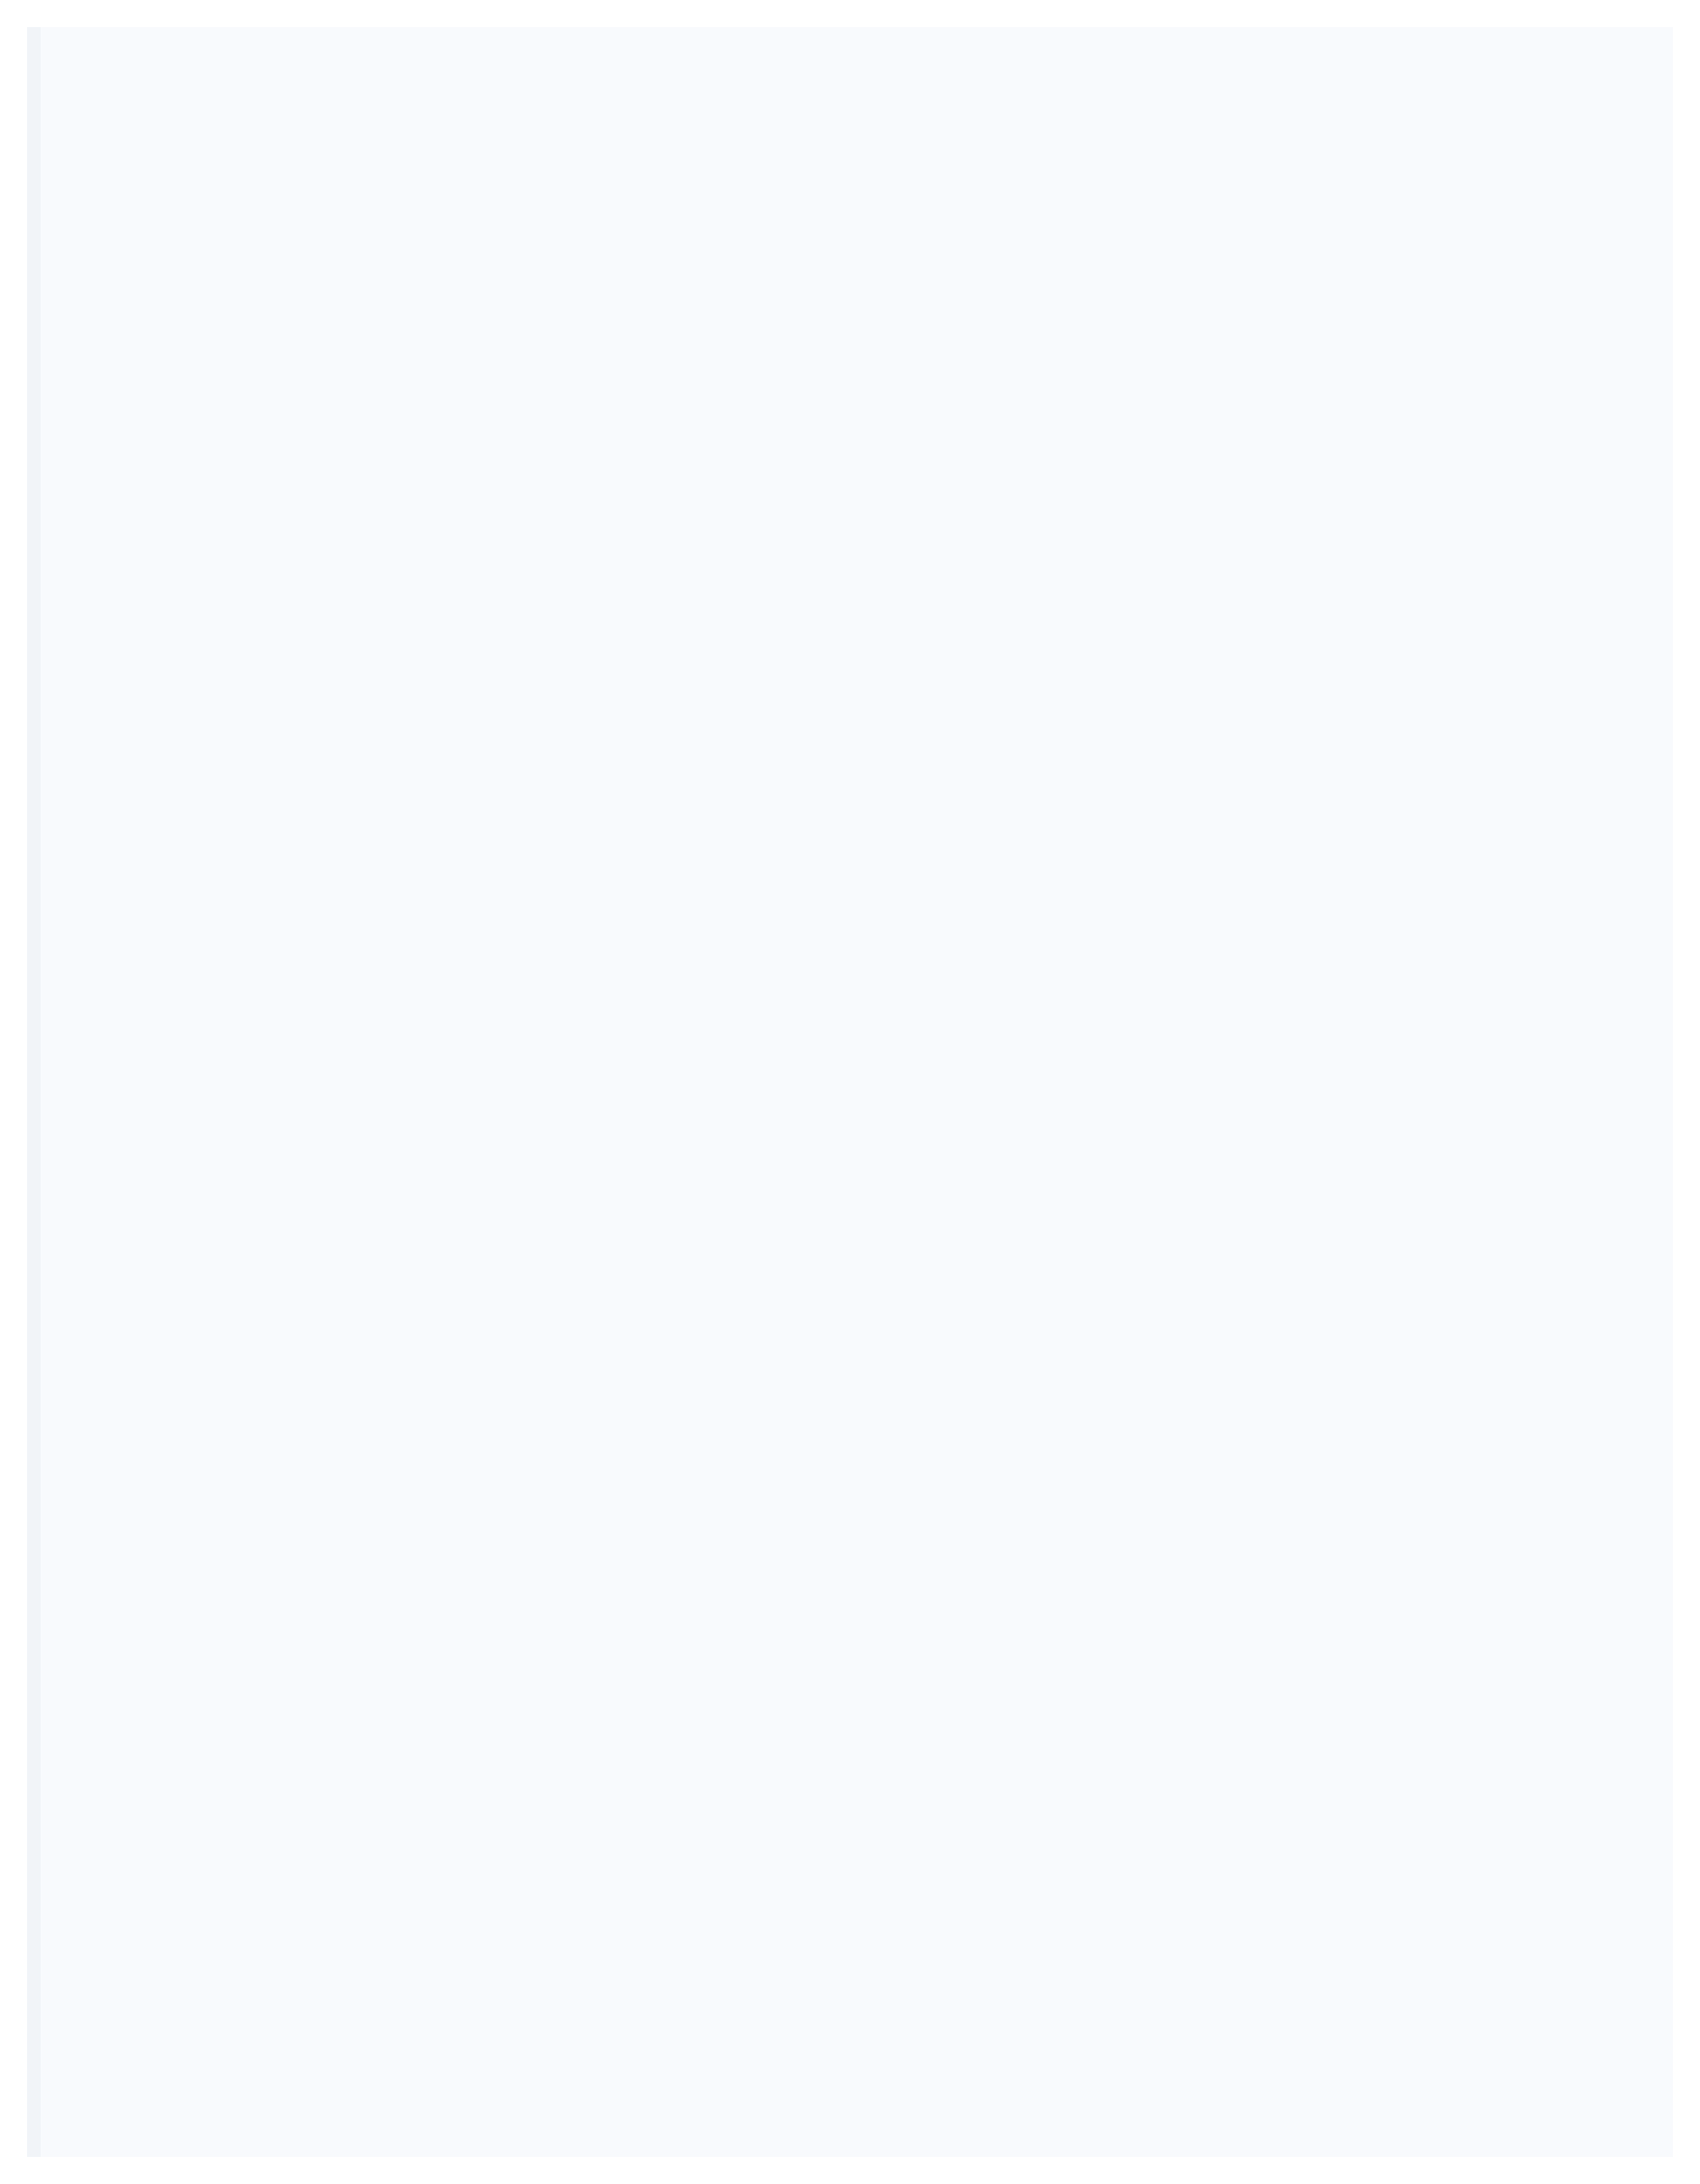
\begin{tikzpicture}
    \useasboundingbox (0,0) rectangle (\paperwidth,\paperheight);
    \fill[slidebg] (0,0) rectangle (\paperwidth,\paperheight);
    \fill[accent!6] (0,0) rectangle (0.18cm,\paperheight);
  \end{tikzpicture}%
}

% ── Background: title / end slides ───────────────────────────
\defbeamertemplate{background canvas}{navybg}{%
  
\begin{tikzpicture}
    \useasboundingbox (0,0) rectangle (\paperwidth,\paperheight);
    \fill[accent]           (0,0) rectangle (\paperwidth,\paperheight);
    \fill[accent!70!black]  (0,0) rectangle (\paperwidth, 0.55cm);
    \foreach \i in {0,0.4,...,4.8}{%
      \draw[white, opacity=0.05, line width=14pt]
        (\paperwidth - \i*1.2cm, \paperheight+0.5cm) --
        (\paperwidth + 1.5cm, \paperheight - \i*1.2cm - 1.5cm);
    }
    \fill[white!15!accent] (0,\paperheight-0.06cm)
      rectangle (\paperwidth,\paperheight);
  \end{tikzpicture}%
}

% ── Frame title ──────────────────────────────────────────────
\setbeamertemplate{frametitle}{%
  \vspace{0.35em}%
  \usebeamerfont{frametitle}\usebeamercolor[fg]{frametitle}%
  \insertframetitle%
  \ifx\insertframesubtitle\@empty\else%
    \hspace{0.6em}{\color{accent!30}\textbar}\hspace{0.5em}%
    \usebeamerfont{framesubtitle}\usebeamercolor[fg]{framesubtitle}%
    \insertframesubtitle%
  \fi%
  \par\vspace{0.2em}%
  {\color{accent!30}\hrule height 0.5pt}%
  \vspace{0.2em}%
}

% ── Footer ───────────────────────────────────────────────────
\setbeamertemplate{footline}{%
  {\color{accent!20}\hrule height 0.4pt}%
  \begin{beamercolorbox}[wd=\paperwidth, ht=0.25cm, dp=0.15cm]{footline}%
    \makebox[\paperwidth]{%
      \hspace{1.0em}%
      {\tiny\color{footergray} Sand Dune \textperiodcentered\ BOS System}%
      \hfill%
      \hspace{-8.0em}%
      {\tiny\color{footergray} Xander Linzel}%
      \hfill%
      {\tiny\color{accent!70}\insertframenumber\,/\,\inserttotalframenumber}%
      \hspace{1.0em}%
    }%
  \end{beamercolorbox}%
}

% ── Title page layout ────────────────────────────────────────
\defbeamertemplate*{title page}{sandune}{%
  \begin{tikzpicture}[overlay, remember picture]
    \fill[white!20!accent]
      ([xshift=1.1cm]current page.west |- current page.north)
      rectangle
      ([xshift=1.45cm]current page.west |- current page.south);
    \node[anchor=west, inner sep=0pt] at
      ([xshift=1.9cm] current page.west |-
       current page.center)
    {%
      \begin{minipage}{0.74\paperwidth}
        \raggedright
        \usebeamerfont{title}\usebeamercolor[fg]{title}\inserttitle
        \par\vspace{-0.35cm}
        {\color{white!40!accentmid}\rule{4.8cm}{1.2pt}}
        \par\vspace{0.4em}
        \usebeamerfont{subtitle}\usebeamercolor[fg]{subtitle}\insertsubtitle
        \par\vspace{1.2em}
        \usebeamerfont{author}\usebeamercolor[fg]{author}\insertauthor
        \par\vspace{0.25em}
        \usebeamerfont{date}\usebeamercolor[fg]{date}\insertdate
      \end{minipage}%
    };
  \end{tikzpicture}%
}

% ── Itemize bullets ──────────────────────────────────────────
\setbeamertemplate{itemize item}  {\footnotesize\raisebox{0.15ex}{\color{accent}$\blacktriangleright$}}
\setbeamertemplate{itemize subitem}{\footnotesize\raisebox{0.15ex}{\color{accentmid}$\triangleright$}}

% ── Blocks ───────────────────────────────────────────────────
\setbeamertemplate{block begin}{%

  \vspace{0.25em}
  \begin{beamercolorbox}[
      rounded=true,
      wd=\linewidth,
      leftskip=0.5em, rightskip=0.5em,
      ht=1.4em, dp=0.3em]{block title}%
    \usebeamerfont{block title}\insertblocktitle
  \end{beamercolorbox}%
  \begin{beamercolorbox}[
      rounded=true,
      wd=\linewidth,
      leftskip=0.6em, rightskip=0.5em, sep=0.35em]{block body}%
    \usebeamerfont{block body}\ignorespaces
}
\setbeamertemplate{block end}{\end{beamercolorbox}\vspace{0.15em}}

\setbeamertemplate{block alerted begin}{%
  \vspace{0.25em}
  \begin{beamercolorbox}[
      rounded=true,
      wd=\linewidth,
      leftskip=0.5em, rightskip=0.5em,
      ht=1.4em, dp=0.3em]{block title alerted}%
    \usebeamerfont{block title}\insertblocktitle
  \end{beamercolorbox}%
  \begin{beamercolorbox}[
      rounded=true,
      wd=\linewidth,
      leftskip=0.6em, rightskip=0.5em, sep=0.35em]{block body alerted}%
    \usebeamerfont{block body}\ignorespaces
}
\setbeamertemplate{block alerted end}{\end{beamercolorbox}\vspace{0.15em}}

% ── Helpers ──────────────────────────────────────────────────
\newcommand{\code}[1]{{\ttfamily\color{accent!85!black}#1}}
\newcommand{\param}[1]{{\ttfamily\color{accent!60!black}#1}}
\newcommand{\theadrow}{\rowcolor{accentlight}}
\setlength{\abovedisplayskip}{3pt}
\setlength{\belowdisplayskip}{3pt}
\setlength{\abovedisplayshortskip}{1pt}
\setlength{\belowdisplayshortskip}{1pt}

% ============================================================
%  METADATA
% ============================================================
\title{Sand Dune}
\subtitle{Design, Modeling, and Validation of a Background Oriented Schlieren System\\[0.2em]
  for High-Resolution Refractive Index Mapping of Transparent Media}
\author{Xander Linzel}
\date{\today}

% ============================================================
\begin{document}
\usebeamerfont{normal text}
% ============================================================

% ── Title ────────────────────────────────────────────────────
{%
  \setbeamertemplate{background canvas}[navybg]%
  \setbeamertemplate{background}{}%
  \setbeamertemplate{footline}{}%
  \begin{frame}[plain]
    \titlepage
  \end{frame}%
}

% ── Outline ──────────────────────────────────────────────────
%\setbeamertemplate{section in toc}{\vspace{0.5em}\inserttocsection}
%\begin{frame}{Outline}
%  \begin{columns}[t]
%    \column{0.25\textwidth}
%      \tableofcontents[sections={1-5}]
%    \column{0.25\textwidth}
%      \tableofcontents[sections={6-10}]
%  \end{columns}
%\end{frame}

% ============================================================
\section{Introduction}
% ============================================================

\begin{frame}{Introduction}{Basis of Background Oriented Schlieren}
  \begin{columns}[t]
    \column{0.52\textwidth}
      \textbf{Core Principle}
      \begin{itemize}
        \item A structured background is imaged \emph{through} a transparent specimen
        \item Refractive-index gradients cause apparent pattern displacements
        \item Comparing reference and disturbed images yields the gradient field
        \item Integrating gradients reconstructs a relative map of $\Delta n$ or $\Delta t$
      \end{itemize}
      \vspace{0.4em}
      \textbf{Advantages}
      \begin{itemize}
        \item Ideal for \emph{weak} disturbances where interferometry is impractical
        \item Non-contact, full-field, and quantitative
        \item Sand Dune implements the \emph{full} measurement chain, optical rig through reconstruction and export
      \end{itemize}
    \column{0.43\textwidth}
      \vspace{-0.5cm}
      \begin{block}{Measurement Pipeline}
        \begin{enumerate}
          \small
          \item Capture \textbf{reference} image (no sample)
          \item Capture \textbf{flow} image (sample present)
          \item Measure pixel \textbf{displacements} via cross-correlation
          \item \textbf{Scale} displacements to physical gradient units
          \item \textbf{Integrate} gradients to obtain RI or thickness map
        \end{enumerate}
      \end{block}
      \vspace{0.3em}
      \small Accuracy is dependent on the \textbf{entire chain}: background design, optical geometry, image quality, sub-pixel estimation, validation, and reconstruction.
  \end{columns}
\end{frame}

% ============================================================
\section{System Design}
% ============================================================

\begin{frame}{System Design}{Optical Layout \& Hardware}
  \begin{columns}[t]
    \column{0.5\textwidth}
      \textbf{Target Regime}\\[0.2em]
      Weak-to-moderate refractive disturbances, sub-pixel displacements sensitive to every stage.

      \vspace{0.35em}
      \textbf{Design Constraints}
      \begin{itemize}
        \item Stable alignment: camera, specimen, background
        \item Repeatable sample positioning
        \item Background texture dense enough for reliable sub-pixel correlation
      \end{itemize}
      \vspace{0.35em}
      \textbf{Key Geometric Parameters}
      \begin{center}
        \small
        \begin{tabular}{cl}
          \toprule
          \theadrow Symbol & Description \\
          \midrule
          $Z_d$    & Background-to-sample distance \\
          $Z_a$    & Sample-to-lens distance \\
          $f$      & Lens focal length \\
          $P_{px}$ & Sensor pixel pitch \\
          \bottomrule
        \end{tabular}
      \end{center}
    \column{0.45\textwidth}
    \vspace{-0.25cm}
      \begin{block}{Hardware Components}
        \begin{itemize}
          \item Camera + 25\,mm fixed focal-length lens
          \item LED backlight panel (incoherent, no speckle)
          \item Blue optical filter (reduces chromatic aberration)
          \item Printed dot-pattern background targets (6 variants)
          \item Rigid support structure
          \item Custom specimen holder for repeatable positioning
        \end{itemize}
      \end{block}
      \vspace{0.3em}
      \small A circular software mask restricts reconstruction to the sample aperture, excluding the holder.
  \end{columns}
\end{frame}


\begin{frame}{System Design}{Optical Layout \& Hardware}

      \begin{figure}[H]
        \centering
            \figimg[width=0.75\linewidth]{hardware_cad.png}
            \caption{Hardware design of Sand Dune optical rig showing camera, lens, specimen region,
                    and patterned background target.}
        \label{fig:hardware}
      \end{figure}
\end{frame}

\begin{frame}{System Design}{Background Pattern Selection}
  \begin{columns}[t]
    \column{0.52\textwidth}
     
    \vspace{0.25cm}
      \textbf{Six Fabricated Patterns}
      \begin{itemize}
        \item Fill densities: \textbf{40\%} and \textbf{60\%}
        \item Dot diameters: 0.10\,mm, 0.50\,mm, 0.75\,mm
      \end{itemize}
      \vspace{0.35em}
      \textbf{Optimal Dot Size: 4--5\,px on sensor}
      \begin{center}
        \small
        \begin{tabular}{cp{5.5cm}}
          \toprule
          \theadrow Size & Effect \\
          \midrule
          $<$3\,px & Under-sampled; narrow noisy peak, poor CMM support \\
          4--5\,px & Well-resolved peak, broad CMM basin, maximum S2N \\
          $>$7\,px & Fewer features per window; lower S/N \\
          \bottomrule
        \end{tabular}
      \end{center}
      \vspace{0.25em}
      \textbf{Current optimum:} 0.10\,mm dots at 40\% density.
    \column{0.43\textwidth}
    
    \vspace{-0.3cm}
      \begin{alertblock}{Illumination}
        \textbf{LED required.} Coherent sources produce speckle, structured noise that degrades sub-pixel accuracy.
      \end{alertblock}
      \vspace{0.3em}
      \begin{alertblock}{Focus}
        Out-of-focus dots blur edges and reduce contrast, degrading the correlation peak shape that CMM relies on. Focus the background as sharply as possible.
      \end{alertblock}
      \vspace{0.3em}
      \small \textbf{Density:} 40\% for large windows/coarse mag; 60\% for small windows or near-lower-bound dot size.
  \end{columns}
\end{frame}

% ============================================================
\section{BOS Measurement Model}
% ============================================================

\begin{frame}{BOS Measurement Model}{What BOS Actually Measures}
  \begin{columns}[t]
    \column{0.5\textwidth}
    \begin{minipage}[t][\columnheight][t]{\linewidth}
    \vspace{0.5cm}
      \textbf{Fundamental Quantity: Optical Path Length}
      \[
        \mathrm{OPL}(x,y) = \int_0^t n(x,y,z)\,dz \approx n(x,y)\cdot t
      \]
      A lateral OPL gradient deflects the ray:
      \[
        \varepsilon_x \approx \frac{t}{n}\,\frac{\partial n}{\partial x}
        \quad\Rightarrow\quad
        u_{px} = \frac{\varepsilon_x Z_d}{P_{px}}\cdot\frac{z_i}{Z_B}
      \]
      \vspace{0.15em}
      \textbf{Two Modes (one quantity must be known):}
      \begin{itemize}
        \item \textbf{dn mode:} $t$ known $\rightarrow$ reconstructs $\Delta n(x,y)$
        \item \textbf{mm mode:} $n$ known $\rightarrow$ reconstructs $\Delta t(x,y)$
      \end{itemize}
      \end{minipage}
    \column{0.45\textwidth}
    
    \vspace{-0.5cm}
      \begin{alertblock}{Fundamental Limitation}
        BOS measures integrated OPL and \emph{cannot} independently separate $n$ and $t$ without additional information (profilometry, OCT, etc.).
      \end{alertblock}
      \vspace{0.3em}
      \textbf{Other Physical Contributors}
      \begin{itemize}
        \item Flat-surface refraction offset (Snell's law, correctable)
        \item Sample tilt, uniform plane in $u$/$v$ maps
        \item Surface curvature and figure errors
        \item Stress birefringence (scalar mean only)
      \end{itemize}
      \vspace{0.25em}
      \small All contributions are integrated into the surface map. Attribution requires independent measurements.
  \end{columns}
\end{frame}

\begin{frame}{BOS Measurement Model}{Scaling \& Geometry}
  \begin{columns}[t]
    \column{0.4\textwidth}
      \textbf{Image distance} (thin-lens, $Z_B = Z_a + Z_d$):
      \[
        z_i = \frac{f\,Z_B}{Z_B - f}
      \]
      \textbf{Correlation-map scale factor (dn mode):}
      \[
        S_{\mathrm{corr}} = P_{px}\,\frac{n\,(Z_B - f)}{f\,Z_d\,t}
        \;\Rightarrow\;
        \frac{\partial n}{\partial x} = u_{px}\cdot S_{\mathrm{corr}}
      \]
      \textbf{Sample-plane grid spacing:}
      \[
        \Delta x_{\mathrm{grid}} = \texttt{step}\cdot P_{px}\cdot\frac{Z_a}{z_i}
      \]
      \textbf{Surface scale factor:}
      \[
        S_{\mathrm{surf}} = S_{\mathrm{corr}}\times\Delta x_{\mathrm{grid}}
      \]
    \column{0.45\textwidth}
      \begin{block}{Optional Refraction Correction (Optional)}
        Off-axis rays through a flat slab shift the apparent background position even for a \emph{uniform} sample.
        \vspace{0.3em}

        Computed via Snell's law and subtracted before scaling:
        \[
          \theta_{r,x} = \arcsin\!\!\left(\tfrac{\sin\theta_x}{n}\right),\quad
          d_x = \frac{\sin(\theta_x - \theta_{r,x})}{\cos\theta_{r,x}}\,t
        \]
        Significant for large $n$ or thick $t$; negligible near $n\approx1$.
      \end{block}
  \end{columns}
\end{frame}

% ============================================================
\section{Processing Pipeline}
% ============================================================

\begin{frame}{Processing Pipeline}{Three-Stage Overview}
  \vspace{0.1em}
  \begin{center}
  \scalebox{0.78}{%
  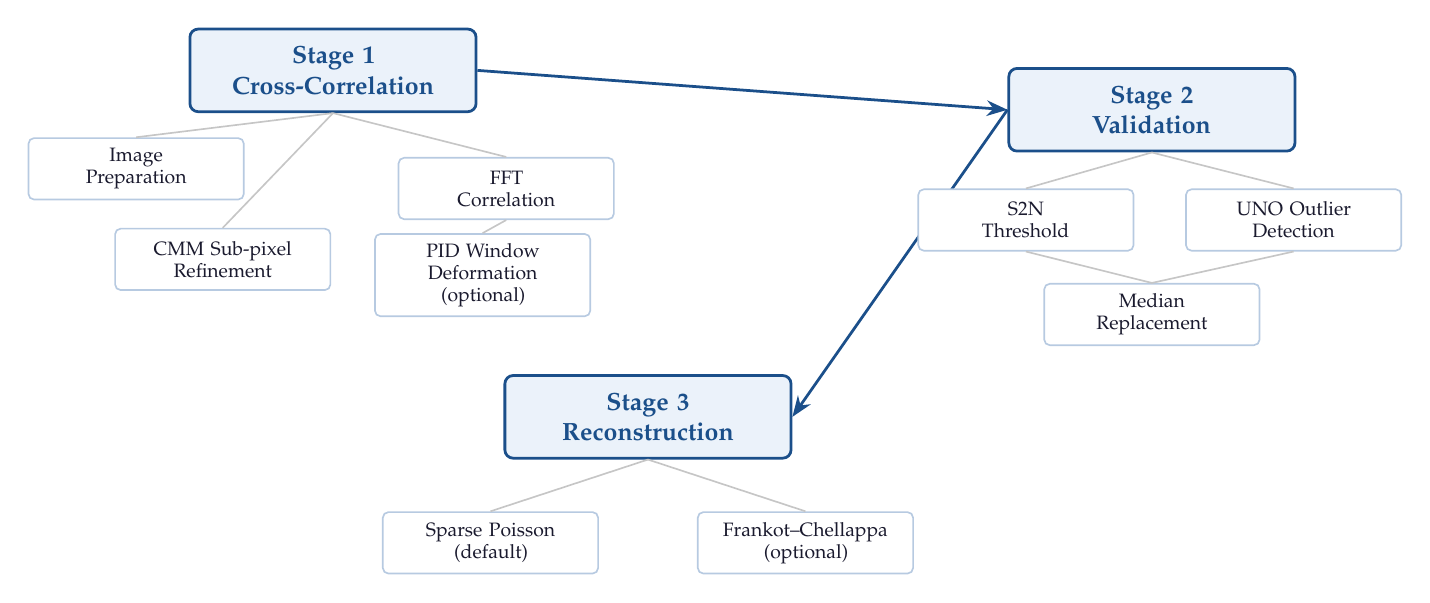
\begin{tikzpicture}[
    box/.style  = {rectangle, rounded corners=3pt, draw=accent, line width=1pt,
                   fill=accentlight, text width=3.4cm, minimum height=1.05cm,
                   align=center, font=\small\bfseries\color{accent}},
    sub/.style  = {rectangle, rounded corners=2pt, draw=accentmid!40, line width=0.6pt,
                   fill=white, text width=2.5cm, minimum height=0.78cm,
                   align=center, font=\scriptsize\color{darktext}},
    arr/.style  = {-Stealth, line width=1pt, color=accent},
    conn/.style = {gray!45, line width=0.6pt},
  ]
    % ── Top row ──────────────────────────────────────────────
    \node[box] (corr)  at (-5.0,  6.0) {Stage 1\\Cross-Correlation};
    \node[box] (val)   at (5.4,  5.5) {Stage 2\\Validation};
    \node[box] (recon) at (-1.0, 1.6) {Stage 3\\Reconstruction};
    \draw[arr] (corr.east)  -- (val.west);
    \draw[arr] (val.west)   -- (recon.east);

    % ── Stage 1 sub-nodes ────────────────────────────────────
    \node[sub] (img) at (-7.5, 4.75) {Image\\Preparation};
    \node[sub] (fft) at ( -2.8, 4.5) {FFT\\Correlation};
    \node[sub] (cmm) at ( -6.4, 3.6) {CMM Sub-pixel\\Refinement};
    \node[sub] (pid) at ( -3.1, 3.4) {PID Window\\Deformation\\(optional)};
    \draw[conn] (corr.south) -- (img.north);
    \draw[conn] (corr.south) -- (fft.north);
    \draw[conn] (corr.south) -- (cmm.north);
    \draw[conn] (fft.south)  -- (pid.north);

    % ── Stage 2 sub-nodes ────────────────────────────────────
    \node[sub] (s2n) at (3.8, 4.1) {S2N\\Threshold};
    \node[sub] (uno) at (7.2, 4.1) {UNO Outlier\\Detection};
    \node[sub] (rep) at (5.4, 2.9){Median\\Replacement};
    \draw[conn] (val.south) -- (s2n.north);
    \draw[conn] (val.south) -- (uno.north);
    \draw[conn] (s2n.south) -- (rep.north);
    \draw[conn] (uno.south) -- (rep.north);

    % ── Stage 3 sub-nodes ────────────────────────────────────
    \node[sub] (sp) at ( -3.0, 0.0) {Sparse Poisson\\(default)};
    \node[sub] (fc) at (1.0, 0.0) {Frankot--Chellappa\\(optional)};
    \draw[conn] (recon.south) -- (sp.north);
    \draw[conn] (recon.south) -- (fc.north);

  \end{tikzpicture}%
  }%
  \end{center}
\end{frame}

\begin{frame}{Processing Pipeline}{Stage 1 --- FFT Cross-Correlation}
  \begin{columns}[t]
    \column{0.5\textwidth}
    
    \begin{minipage}[t][\columnheight][t]{\linewidth}
    \vspace{-2cm}
      \textbf{Window Grid} \;($W$ = window size, $O$ = overlap)
      \[
        \texttt{step} =  W - O \quad
        n_c = \left\lfloor\frac{W_\mathrm{img}-W}{\texttt{step}}\right\rfloor+1
      \]
      \textbf{Per-Window Steps}
      \begin{enumerate}
        \small
        \item Extract reference and flow interrogation blocks
        \item Skip if local variance $< 10^{-3}$ (flat patch)
        \item Subtract local mean
        \item Forward FFT of both windows
        \item Cross-power spectrum $G = \overline{F_\mathrm{ref}}\,F_\mathrm{flow}$
        \item Inverse FFT $\to$ correlation map $\phi$; shift to centre
      \end{enumerate}
      \[
        \phi = \mathcal{F}^{-1}\!\left\{\overline{F_{\mathrm{ref}}}\,F_{\mathrm{flow}}\right\}
      \]
    \end{minipage}
    \column{0.45\textwidth}
    \begin{minipage}[t][\columnheight][t]{\linewidth}
    \vspace{-1.5cm}
      \textbf{Signal-to-Noise Ratio}
      \[
        \mathrm{s2n} = \frac{\phi_1}{\phi_2}
      \]
      \small $\phi_1$: primary peak; \;$\phi_2$: highest value outside $\pm2$\,px exclusion zone.

      \vspace{0.4em}
      \begin{block}{FFTW Implementation}
        FFTW3 (single-precision float) plans allocated once at \code{Correlator} construction and reused across all windows, avoiding per-frame planning overhead.
      \end{block}
    \end{minipage}
  \end{columns}
\end{frame}

\begin{frame}{Processing Pipeline}{Stage 1 --- CMM Sub-Pixel Refinement}
  \begin{columns}[t]
    \column{0.52\textwidth}
      \textbf{Correlation Mapping Method} \small(Chen \& Katz, 2005)
      \begin{itemize}
        \item $5\times5$ patch centred on the discrete correlation peak
        \item Minimises mean-normalised residual against the autocorrelation:
          \[
            \varepsilon = \sum_{i=0}^{24}\!\left(\tilde{\phi}[i] - \tilde{\phi}'[i]\right)^2
          \]
        \item $\tilde{\phi}'$ evaluated at offset $(u',v')$ via bicubic interpolation
      \end{itemize}
      \textbf{Solver Sequence}
      \begin{enumerate}
        \small
        \item \textbf{Seed:} log-parabola fit along dominant axis
        \item \textbf{Gauss--Newton:} $\leq$8 iters, backtracking line-search
        \item \textbf{Grid fallback:} dense 0.01\,px search if G--N fails
        \item \textbf{Boundary handoff:} test adjacent cell if within 0.02\,px of $\pm0.5$
      \end{enumerate}
      \small Solution clamped to $|u'|,|v'|\leq0.49$\,px.
    \column{0.43\textwidth}
      \begin{alertblock}{Peak Locking Suppression}
        Centroid/parabola fits are biased toward integer values, producing artefact spikes in displacement histograms.

        \vspace{0.3em}
        CMM fits the \emph{entire patch shape}, not just the peak tip, suppressing this bias. Boundary-handoff and the $\pm0.49$ clamp are additional safeguards.
      \end{alertblock}
  \end{columns}
\end{frame}

\begin{frame}{Processing Pipeline}{Stage 1 --- CMM Sub-Pixel Refinement}
  
      \begin{figure}[H]
        \centering
            \figimg[width=0.43\linewidth]{peak_locking.png}
            \caption{Peak locking when using gaussian interpolation for sub-pixel displacement.}
        \label{fig:hardware}
      \end{figure}

\end{frame}

\begin{frame}{Processing Pipeline}{Stage 1 --- Progressive Image Deformation (PID)}
  \begin{columns}[t]
    \column{0.52\textwidth}
    
    \begin{minipage}[t][\columnheight][t]{\linewidth}
    \vspace{0.4cm}
      \textbf{Motivation:} rigid windows ignore local shear and strain, biasing the displacement estimate for non-uniform fields.

      \vspace{0.3em}
      \textbf{Algorithm (per PID pass)}
      \begin{enumerate}
        \small
        \item Compute 1st-order displacement gradients via central differences
        \item Apply $3\times3$ box-filter smoothing (\param{pid\_smoothing\_passes})
        \item Build affine warp at each window centre
        \item Resample flow window; re-correlate for residual
        \item Accept update only if CMM residual improves
        \item Repeat; stop early if mean correction $<10^{-3}$\,px
      \end{enumerate}
      
    \end{minipage}
    \column{0.43\textwidth}
    \vspace{-0.25cm}
      \begin{block}{Parameters}
        \small
        \begin{tabular}{ll}
          \param{enable\_pid}           & on/off \\
          \param{pid\_iterations}       & \# PID passes \\
          \param{pid\_relaxation}       & damping $\in[0,1]$ \\
          \param{pid\_smoothing\_passes}& filter count \\
        \end{tabular}
      \end{block}
      \vspace{0.3em}
      \textbf{Measured Benefit} (affine test field)
      \begin{center}
        \small
        \begin{tabular}{lc}
          \toprule
          \theadrow Method & RMSE (px) \\
          \midrule
          Baseline (no PID)  & 0.2745 \\
          PID - 2 iters    & 0.0875 \\
          PID - 3 iters    & 0.0846 \\
          \bottomrule
        \end{tabular}
      \end{center}
      \small 2 passes give $\mathbf{68\%}$ RMSE reduction; 3rd adds only $3\%$.
  \end{columns}
\end{frame}

\begin{frame}{Processing Pipeline}{Stage 2 --- Validation}
  \begin{columns}[t]
    \column{0.5\textwidth}
    
    \begin{minipage}[t][\columnheight][t]{\linewidth}
    \vspace{-1.5cm}
      \textbf{Pass 1: Signal-to-Noise Threshold}
      \[
        \text{Flag if} \quad \mathrm{s2n} < 1.3
      \]
      \textbf{Pass 2: Universal Normalized Residual (UNO)}
      \small(Westerweel \& Scarano, 2005)
      \[
        \tilde{u}_{\mathrm{nrm}} =
          \frac{|u - u_{\mathrm{med}}|}
               {\mathrm{median}(|u_k - u_{\mathrm{med}}|) + 0.1}
      \]
      \[
        \text{Flag if} \quad
        \sqrt{\tilde{u}_{\mathrm{nrm}}^2 + \tilde{v}_{\mathrm{nrm}}^2} > 2.0
      \]
      \small $u_{\mathrm{med}}$: 8-connected neighbourhood median.

      \vspace{0.3em}
      \textbf{Replacement:} flagged vectors $\rightarrow$ 8-neighbourhood median of unflagged neighbours.
      \end{minipage}
    \column{0.45\textwidth}
    \vspace{-0.5cm}
      \begin{block}{UNO Purpose}
        The normalised residual adapts to local displacement magnitude, unlike a fixed absolute threshold, it remains effective across spatially varying signal levels.
      \end{block}
      \vspace{0.3em}
  \end{columns}
\end{frame}

\begin{frame}{Processing Pipeline}{Stage 3 --- Surface Reconstruction}
  \begin{columns}[t]
    \column{0.5\textwidth}
    \begin{minipage}[t][\columnheight][t]{\linewidth}
    \vspace{0.8cm}
      \textbf{Default: Masked Sparse Poisson Solver}\\[0.2em]
      Minimise edge-gradient energy over masked valid nodes:
      \[
        E(s) = \!\!\sum_{\text{x-edges}}\!\!\left(s_{i,j+1} - s_{i,j} - g^x_{i,j}\right)^2
              \!+\!\!\sum_{\text{y-edges}}\!\!\left(s_{i+1,j} - s_{i,j} - g^y_{i,j}\right)^2
      \]
      \small where $g^x_{i,j} = \tfrac{1}{2}(u_{i,j}+u_{i,j+1})$.
      Setting $\partial E/\partial s_{i,j}=0$ yields a sparse system solved with \code{Eigen::ConjugateGradient}. First valid node pinned to zero.
    \end{minipage}
    \column{0.45\textwidth}
      \begin{block}{Frankot--Chellappa (Optional)}
        FFT-based frequency-domain integration:
        \[
          \hat{s} =
          \frac{if_x\hat{u} + if_y\hat{v}}{2\pi(f_x^2+f_y^2)+\varepsilon}
        \]
        Much faster but zeroing gradients outside the mask can introduce boundary artifacts on heavy masks.
      \end{block}
      \vspace{0.3em}
      \small \textbf{Recommendation:} Sparse Poisson for masked datasets; Frankot--Chellappa for fast comparison on full-domain fields.
  \end{columns}
\end{frame}

% ============================================================
\section{Software Architecture}
% ============================================================

\begin{frame}{Software Architecture}{Build System \& Key Classes}
  \begin{columns}[t]
    \column{0.47\textwidth}
      \textbf{Build: CMake, C++23.}
      Targets: \code{sand\_dune} (GUI) and \code{run\_tests} (test binary).
      \vspace{0.3em}
      \begin{center}
        \small
        \begin{tabular}{ll}
          \toprule
          \theadrow Library & Role \\
          \midrule
          SDL3, SDL3\_image  & Window, render, image I/O \\
          Dear ImGui         & All UI panels \& controls \\
          ImPlot             & Heatmap visualisations \\
          Eigen3             & Dense/sparse linear algebra \\
          FFTW3 (float)      & FFT correlation \& FC \\
          doctest            & Unit-test framework \\
          \bottomrule
        \end{tabular}
      \end{center}
    \column{0.48\textwidth}
      \textbf{Key Classes}
      \begin{itemize}
        \item \textbf{\code{Session}}: orchestrator; owns images, intermediate arrays, parameter structs, and async stage-state machine (\code{std::atomic<StageState>})
        \item \textbf{\code{Correlator}}: reference + flow $\to$ \code{VectorField}; FFTW plans allocated once at construction
        \item \textbf{\code{Reconstruction}}: sparse Poisson and Frankot--Chellappa back ends
        \item \textbf{\code{VectorField}}: stores $u$, $v$, s2n matrices; exposes \code{SaveCSV()}
        \item \textbf{\code{Image}}: normalized $[0,1]$ float matrix loader
      \end{itemize}
      \small Stages run via \code{std::async}; UI polls stage states to update progress.
  \end{columns}
\end{frame}

% ============================================================
\section{Using the Application}
% ============================================================

\begin{frame}{Using the Application}{Typical Workflow}
  \begin{enumerate}
    \small
    \item[\textbf{1.}] \textbf{Load images}: Reference + one or more flow images via the \textbf{Load} panel. All images must share identical pixel dimensions.
    \vspace{0.2em}
    \item[\textbf{2.}] \textbf{Set parameters}: Optical geometry ($Z_d$, $Z_a$, $f$, $P_{px}$), sample properties ($n$, $t$), correlation settings. The \textbf{Calculations} panel updates live with derived grid spacing, physical field width, and feature size estimate.
    \vspace{0.2em}
    \item[\textbf{3.}] \textbf{Configure the mask}: Enable circular mask; set centre and radius to enclose the sample region.
    \vspace{0.2em}
    \item[\textbf{4.}] \textbf{Run pipeline}: \textbf{Run Full Pipeline} (all three stages) or each stage individually. Progress bar and ETA shown per stage.
    \vspace{0.2em}
    \item[\textbf{5.}] \textbf{Inspect results}: Correlation, Validation, and Surface tabs; toggle raw pixel / physical units; adjust colormap via min/max sliders.
    \vspace{0.2em}
    \item[\textbf{6.}] \textbf{Export}: Choose output directory in the \textbf{Save} panel. Three CSV files per frame: \texttt{\_correlation.csv}, \texttt{\_val.csv}, \texttt{\_surface.csv}.
  \end{enumerate}
\end{frame}

\begin{frame}{Using the Application}{Parameters Panel Reference}
  \begin{center}
    \small
    \begin{tabular}{llp{7.2cm}}
      \toprule
      \theadrow Group & Control & Effect \\
      \midrule
      Correlation & Window size       & Interrogation window side length (px) \\
                  & Overlap           & Window overlap; $\texttt{step}=W-O$ \\
                  & Enable PID        & Iterative window deformation \\
                  & PID iterations    & Number of passes after baseline \\
                  & PID relaxation    & Damping on residual updates $[0,1]$ \\
      \midrule
      Optical     & $P_{px}$          & Sensor pixel pitch (\si{\micro\metre}) \\
                  & $Z_d$, $Z_a$, $f$ & Geometry distances (\si{mm}) \\
      \midrule
      Sample      & $n$, $t$          & Refractive index and thickness (\si{mm}) \\
      \midrule
      Reconstruction & Mode           & RI variation (dn) or thickness variation (mm) \\
                     & Apply correction & Subtract Snell's-law geometric offset \\
      \midrule
      Mask        & Enable / Centre / Radius & Restrict reconstruction to circular ROI \\
      \bottomrule
    \end{tabular}
  \end{center}
\end{frame}

% ============================================================
\section{Validation \& Precision}
% ============================================================

\begin{frame}{Validation \& Precision}{Image-Based Precision Metric}
  \begin{columns}[t]
    \column{0.5\textwidth}
      \textbf{Test Image Pair: \texttt{if\_0.1}}\\
      Glass window of \emph{known uniform} RI and thickness. Expected field: smooth, nearly planar, plane-fit residual quantifies spurious structure (striping, locking artifacts).

      \vspace{0.3em}
      \begin{center}
        \small
        \begin{tabular}{lcc}
          \toprule
          \theadrow Metric & $u$ (px) & $v$ (px) \\
          \midrule
          Whole-map, no PID    & 0.659 & 0.670 \\
          Whole-map, PID       & 0.596 & 0.579 \\
          Central crop, no PID & 0.096 & 0.106 \\
          \textbf{Central crop, PID} & \textbf{0.049} & \textbf{0.046} \\
          \bottomrule
        \end{tabular}
      \end{center}
      \small Central crop = inner 80\%; outer 10\% per side excluded (edge artifacts).
    \column{0.45\textwidth}
      \textbf{PID Improvement on Central Crop}
      \begin{itemize}
        \item $\approx\mathbf{49.5\%}$ reduction in $u$-RMS
        \item $\approx\mathbf{56.8\%}$ reduction in $v$-RMS
      \end{itemize}
      \vspace{0.3em}
      \begin{block}{Additional Diagnostics}
        \textbf{Striping:} for \texttt{if\_0.1}, dominant-axis correlation was $0.9985$ ($u$) and $0.9981$ ($v$); orthogonal-axis correlation was $0.0052$ and $0.0068$.
    
        \vspace{0.25em}
        \textbf{Peak-locking:} half-pixel locked fraction was $0.0430$/$0.0436$ raw and $0.0425$/$0.0431$ validated for $u$/$v$.
    
        \vspace{0.25em}
        \textbf{Residual ratio:} decreased from $0.0517 \rightarrow 0.0505$ in $u$ and $0.0554 \rightarrow 0.0538$ in $v$ after validation.
      \end{block}

  \end{columns}
\end{frame}


\begin{frame}{Validation \& Precision}{Image-Based Precision Metric}
  
      \begin{figure}[H]
        \centering
            \figimg[width=0.43\linewidth]{gradient.png}
            \caption{Optical window measured using BOS system.}
        \label{fig:hardware}
      \end{figure}

\end{frame}

% ============================================================
\section{System Precision Estimate}
% ============================================================

\begin{frame}{System Precision Estimate}{Minimum Resolvable Gradient}
  \begin{columns}[t]
    \column{0.48\textwidth}
      \textbf{Current Optical Configuration}
      \begin{center}
        \small
        \begin{tabular}{llr}
          \toprule
          \theadrow Parameter & Symbol & Value \\
          \midrule
          Focal length       & $f$      & 25\,mm \\
          BG--sample dist.   & $Z_d$    & 220\,mm \\
          Sample--lens dist. & $Z_a$    & 45\,mm \\
          Total obj.\ dist.  & $Z_B$    & 265\,mm \\
          Pixel pitch        & $P_{px}$ & 2.315\,\si{\micro\metre} \\
          Sample RI          & $n$      & 1.08 \\
          Thickness          & $t$      & 0.924\,mm \\
          \bottomrule
        \end{tabular}
      \end{center}
    \column{0.47\textwidth}
      \textbf{Min.\ detectable displacement} ($3\sigma$):
      \[
        u_{\min} = 3\times0.049 \approx 0.15~\text{px}
      \]
      $S_{\mathrm{corr}} \approx 0.1181~\mathrm{m}^{-1}\mathrm{px}^{-1}$

      \textbf{Min.\ resolvable gradient:}
      \[
        \left.\tfrac{dn}{dx}\right|_{\!\min} \approx 1.77\times10^{-5}~\mathrm{dn/mm}
      \]
      \textbf{Worst-case expected} ($\Delta n{=}0.005$ over 24\,mm):
      \[
        \left.\tfrac{dn}{dx}\right|_{\!\mathrm{wc}} \approx 2.08\times10^{-4}~\mathrm{dn/mm}
      \]
      \[
        \textbf{Detection margin} \approx \mathbf{11.8\times}
      \]
      \small Even in the shallowest expected gradient, the system resolves the signal by $\sim$one order of magnitude.
  \end{columns}
\end{frame}

% ============================================================
\section{Calibration}
% ============================================================

\begin{frame}{Calibration \& Interpretation}{}
  \begin{columns}[t]
    \column{0.5\textwidth}
      \textbf{Calibrating $Z_a$}\\
      Most sensitive parameter: an error in $Z_a$ shifts \emph{both} the displayed field width and the reconstructed surface amplitude (both depend on $\Delta x_\mathrm{grid}$).

      \vspace{0.3em}
      \textbf{Do not use a ruler directly.} Recommended procedure:
      \begin{enumerate}
        \small
        \item Place a target of \textbf{known physical width} in the background plane
        \item Record how many pixels span that width
        \item Back-calculate $Z_a$ until the \textbf{Calculations} panel field width matches the known dimension
      \end{enumerate}
      \vspace{0.3em}
      \small The reconstructed surface has an arbitrary constant offset; absolute comparisons across experiments require an independent reference point.
    \column{0.45\textwidth}
      \begin{block}{Reconstruction vs.\ Gradient Maps}
        \textbf{Use the surface map to:}\\
        Characterise overall uniformity; quantify large-scale RI or thickness variation; compare samples.

        \vspace{0.3em}
        \textbf{Use the $u$/$v$ gradient maps to:}\\
        Locate localised defects --- inclusions, bubbles, cracks, steep-gradient regions --- that may be smeared or suppressed by the integration step.

        \vspace{0.3em}
        \emph{Always inspect both together.}
      \end{block}
  \end{columns}
\end{frame}

% ============================================================
\section{Known Caveats}
% ============================================================

\begin{frame}{Known Caveats}{Fundamental \& Software Limitations}
  \begin{columns}[t]
    \column{0.5\textwidth}
      \textbf{Measurement Fundamentals}
      \begin{itemize}
        \item \textbf{$n$ and $t$ cannot be decoupled} from BOS data alone
        \item \textbf{Not a pure RI map}: tilt, curvature, birefringence all contribute
        \item \textbf{Line-of-sight integrated}: 3D depth structure not resolved
        \item \textbf{$\partial n/\partial z$ invisible}: only transverse gradients deflect rays
        \item \textbf{Gradient, not a surface}: integration accumulates errors; inspect both maps
        \item \textbf{Small-angle approx}: breaks down for large deflections
        \item \textbf{Reference must be distortion-free}: lens distortion appears as a systematic offset
      \end{itemize}
    \column{0.45\textwidth}
      \textbf{Software \& Implementation}
      \begin{itemize}
        \item \textbf{Curl-free assumption}: Poisson solver discards non-integrable curl silently; high-curl field can look deceptively smooth
        \item \textbf{FC mask treatment} weaker than sparse Poisson for masked domains
        \item \textbf{Surface is relative}: gauge constant is arbitrary
        \item \textbf{Validation not uniformly applied}: some overloads use S2N pass only
        \item \textbf{Geometry calibration critical}: incorrect $Z_a$ shifts both field width and amplitude by the same factor
      \end{itemize}
  \end{columns}
\end{frame}

% ── Conclusion ───────────────────────────────────────────────
\begin{frame}{Conclusion}{}
  \begin{columns}[t]
    \column{0.54\textwidth}
      \vspace{0.5cm}
      \textbf{Sand Dune} is a complete BOS measurement system for mapping weak optical non-uniformities in transparent media at high spatial resolution.

      \vspace{0.35em}
      \textbf{Key Capabilities}
      \begin{itemize}
        \item FFT cross-correlation + CMM sub-pixel refinement
        \item Optional PID window deformation ($\sim50\%$ precision improvement)
        \item UNO-based two-pass vector validation
        \item Masked sparse Poisson (default) and Frankot--Chellappa (alternative)
        \item Real-time parameter calculations and interactive heatmap visualisation
        \item CSV export for all pipeline stages
      \end{itemize}
      \vspace{0.3em}
      \textbf{Current Precision Benchmark}\\
      Central-crop plane-fit RMS with PID:\\
      $\approx0.049$\,px ($u$) and $0.046$\,px ($v$)
    \column{0.41\textwidth}
      \vspace{-0.5cm}
      \begin{block}{Detection Margin}
        \centering\large
        $\mathbf{11.8\times}$ margin over worst-case gradient.
      \end{block}
      \vspace{0.35em}
      \begin{alertblock}{Next Steps}
        \begin{itemize}
          \item Final experimental repeatability figures
          \item Completed geometry-calibration results
          \item Full hardware-to-absolute-scale documentation
        \end{itemize}
      \end{alertblock}
      \vspace{0.35em}
      \footnotesize \textbf{Refs:} Raffel (2015) $\cdot$ Chen \& Katz (2005) $\cdot$ Westerweel \& Scarano (2005) $\cdot$ Frankot \& Chellappa (1988) $\cdot$ Agrawal et al.\ (2006) $\cdot$ Liu et al.\ (2022)
  \end{columns}
\end{frame}

% ── End slide ────────────────────────────────────────────────
{%
  \setbeamertemplate{background canvas}[navybg]%
  \setbeamertemplate{background}{}%
  \setbeamertemplate{footline}{}%
  \begin{frame}[plain]
    \begin{tikzpicture}[overlay, remember picture]
      \fill[white!20!accent]
        ([xshift=1.1cm]current page.west |- current page.north)
        rectangle
        ([xshift=1.45cm]current page.west |- current page.south);
      \node[anchor=center] at (current page.center) {%
        \begin{minipage}{0.55\paperwidth}
          \centering
          {\color{white}\small Xander Linzel}\\[0.2em]
          {\color{white!75!accent}\footnotesize\ttfamily
            xander.linzel@irradiant.tech}
        \end{minipage}%
      };
    \end{tikzpicture}
  \end{frame}%
}

\end{document}